The tracking sub-detectors are responsible for registering spacial coordinates of charged particles.
The coordinates from multiple layers of tracking sub-systems are processed by the tracking algorithms
to produce {\it tracks}, which are objects representing the trajectory of a charged particle. There are
three distinct tracking sub-detectors in \lhcb shown in \figref{lhcb_detector_cross_section}; Closest to the interaction point is
the {\it VErtex LOcator}, \velo, then just before the \lhcb magnet is the {\it Tracking Turisensis}, \ttracker,
and  lastly the {\it Outer Tracker} \ot. There are several track types that are {\it reconstructed} by
the tracking algorithms, depending on which of the tracking sub-detectors provided information to produce
the track object. The varius track types are shown in \figref{track_types}. The most common tracks used are {\it long}
which have the highest momentum resolution. The overal reconstruction efficiency of long tracks is $\sim 96\%$.

\begin{figure}[t]
  \centering
  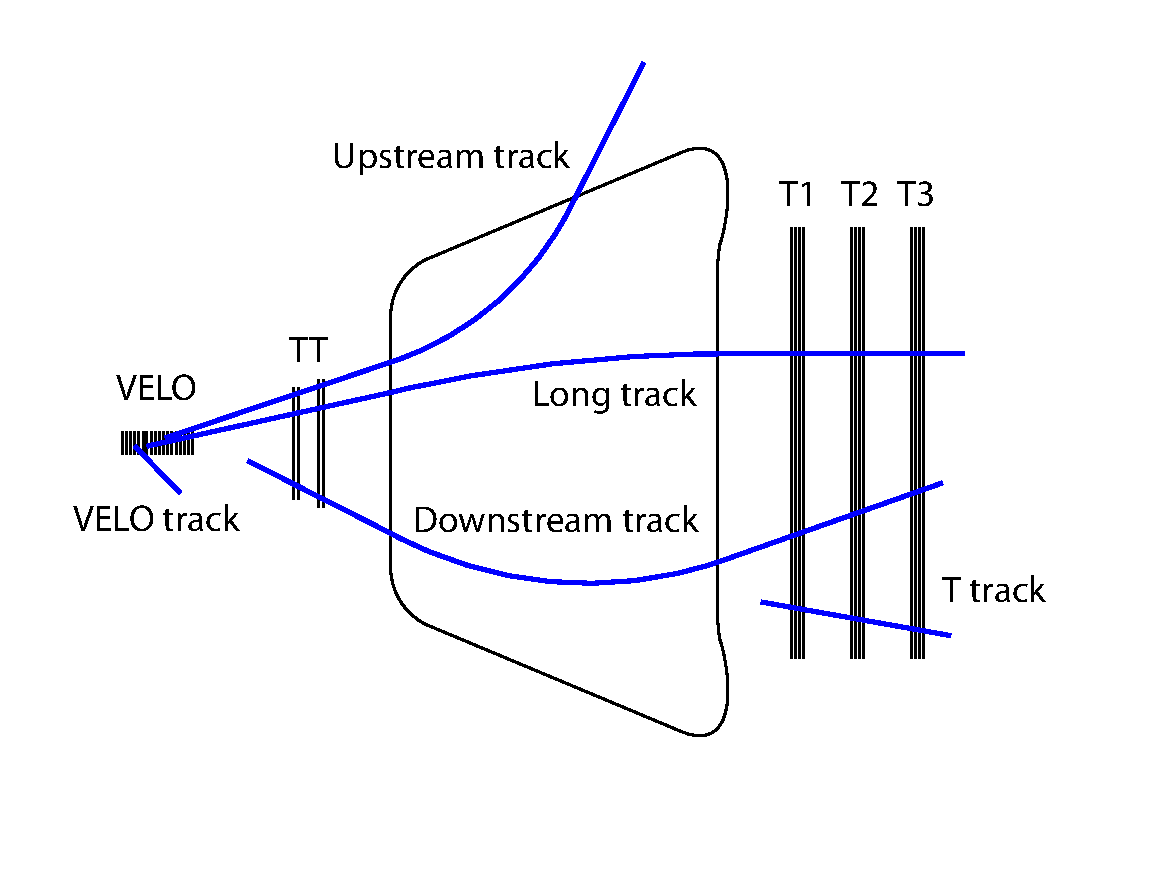
\includegraphics[width=0.7\textwidth]{Figures/Chapter2/trackTypesRunIAndII}
  \caption{\lhcb track types.}
  \label{track_types}
\end{figure}

A charged particle that traverses the \lhcb magnet is deflected. The amount of deflection is inversly proportional
to its momentum. The latter is exploited by tracking algorithms to estimate the momentum of a track. The relative
momentum momentum resolution of the tracking sytem, shown in \figref{det_deltappvp}, is $\nicefrac{\Delta p}{p} \sim 0.5 \%$
for low mementum tracks and up to $1\%$ for 200\gevc momentim tracks. Intuitively, tracks that do not deflect a
lot have inferior momentum resolution.

Measuring the mass of a particle, like the \Bs meson, is achieved by combining tracks in order to build a complete
cascade of partcile decays (also refered to as {\it decay chanell}). The mass measurement presicion varies depending
on the specific decay chanell. Two body \B decays including a \jpsi have the most precise mass resolution of about
$8 \mevcc$. On the other hand decay chanells including neutral particles, \ie $\Bs\to\phi\gamma$, have a worst resolution of
about $100 \mevcc$. Note that neutral particles are undetected by the tracking system. Instead the calorimetry,
introduced in \secref{det_calo}, system is responsible for reconstructing these type of particles.

\begin{figure}[t]
  \centering
  \begin{subfigure}{0.5\textwidth}
    \raggedright
    \includegraphics[width=\textwidth]{Figures/Chapter2/dppVsp-crop-cmyk}
    \caption{}
    \label{det_deltappvp}
  \end{subfigure}%
  \begin{subfigure}{0.5\textwidth}
    \raggedleft
    \includegraphics[width=\textwidth]{Figures/Chapter2/DataResXY_1PV_2012-crop-cmyk.pdf}
    \caption{}
    \label{det_velo_pv_res}
  \end{subfigure}
  \caption{ trigger scheams.}
  \label{det_velo_perf}
\end{figure}

Certain important analysis performed with the \lhcb detector rely on measuring the {\it flight distance} of a particle, like the \Bs meson.
Flight distance is typically the distance between the point were the two protons colideed, called {\it Primary Vertex} (PV)
and the point were the \Bs, in that case, decayed. This last point is called {\it Secondary Vertex} (SV). The \velo sub-detector
was designed for optimum spacial resolution, by placing the \velo sensors as close to the beam as posible, $\sim 8 \mm$.
The PV position resolution depends strongly on the number of tracks used to build the vertex and can be seen in \figref{det_velo_pv_res}.
Measuring the flight distance translates to a {\it decay time} time measurement. The latter is the time interval between
the production and decay of a particle and it is the actual quantity that a typical {\it time dependant} analysis,
\eg \BsJpsiPhi, requires. The average decay time resolution measured with the above channel is $\sim 45\fs$, which
implies that the \phis measurement discussed in \secref{measuring_phis}, is indded posibe to perform.

Lastly, a big part of the \lhcb physics program includes muons. The muon system cositis of {\it Multi Wire Proportional Chambers}
(MWPC). It is positioned after the calorimeters, with the exception of the first, M1, muon station.
Note that muons can penetrate through a large volume of led, like the one present in the calorimeter system,
without decaying. There are 5 muons stations in total; Each station is devided in 4 concentric regions.
The granularity\footnote{In this context granularity is essentially the distance between the wires of the MWPC.}
of each station becomes progresively smaller as one moves towards the inner regions which are closer to the beam pipe.
This is done to acount for the increasing track density that is typicaly found in the forward region. This way
the special resolution is higher exactly where it is needed. The $x$ coordinate hit resolution in all regions
is superior comapred to the $y$ coordinate; Since the configuration direction of the \lhcb magnetic field streangth
is such that tracks bend only along the $x$ plane. The $(x,y)$ resolution varies from $(4,10)\mm$ to $(150,180)\mm$
respectivelly fro the inner M1 region and the outer M5 region. The overal detector efficiency is $\>98\%$.
